\documentclass[12pt]{article}

\usepackage[margin=1in]{geometry}
\usepackage{amsmath,amsthm,amssymb}
\usepackage{nccmath}
\usepackage{mathtools}
\usepackage{mathrsfs}
\usepackage{enumitem}
\usepackage{physics}
\usepackage{slashed}
\usepackage{pdfpages}

\begin{document}

\title{Homework 1}
\author{Sean Ericson \\ Phys 662}
\maketitle
\section*{Problem 1 (Peskin 15.2)}
(See attached Mathematica printout for calculations)
\begin{enumerate}[label=(\alph*)]
    \item Equation (15.40) for the rate of muon decay is 
    \[ \Gamma = \frac{G_F^2m_\mu^5}{192\pi^3}. \]
    The calculation for tau decay rate is identical (assuming we neglect the electron and muon masses). Therefore, substituting the tau mass for the muon's, we find
    \[ \Gamma(\tau \to \nu_\tau \mu^- \bar{\nu}_\mu) = \Gamma(\tau \to \nu_\tau e^- \bar{\nu}_e) = 4.0476 \times 10^{-13} \;\text{GeV} \]
    \item For the given hadronic decay mode, we need to average over the color of the final quarks. The final state is a color singlet, so there's only one color degree of freedom. Therefore, the color average amounts to dividing by 3. Using a value of 0.31 for the strong force at the mass of the tau, we find
    \[ \Gamma(\tau \to \nu_\tau d\bar{u}) \approx \frac{1}{3}\Gamma_l\left(1 + \frac{\alpha_s(m_\tau)}{\pi}\right) = 1.4823 \times 10^{-13} \;\text{GeV} \] 
    \item The total rate is given by
    \[ \Gamma_\text{total} = 2\Gamma_l + \Gamma_h = 2.1436 \times 10^{-12} \;\text{GeV}. \]
    The branching ratio to leptonic modes is
    \[ \text{BR}(\tau \to \nu_\tau l^- \bar{\nu}_l) = \frac{2\Gamma_l}{\Gamma_\text{total}} = 37.76\%, \]
    and the lifetime is
    \[ \tau(\tau) = \frac{\hbar}{\Gamma_\text{total}} = 3.0706 \times 10^{-13} \;\text{s}. \]
    The PDG gives the following values for the branching ration and lifetime:
    \begin{align}
        \text{BR}(\tau \to \nu_\tau\mu^-\bar{\nu}_\mu) &= (17.3937\pm0.0384)\% \\
        \text{BR}(\tau \to \nu_\tau e^- \bar{\nu}_e) &= (17.8175\pm0.0399)\% \\
        \implies \; \text{BR}(\tau \to \nu_\tau l^- \bar{\nu}_l) &= (35.2112\pm0.0783)\% \\
        \tau(\tau) &= (2.903 \pm0.005)  \times 10^{-13} \;\text{s}
    \end{align}
    Very close!
\end{enumerate}


\section*{Problem 2}
The full lagrangian is
\[ \mathscr{L} = i\bar{\Psi}\slashed{D}\Psi - \left(D_\mu\phi\right)^\dag D^\mu\phi - \frac{1}{4}F_{\mu\nu}F^{\mu\nu} - \lambda\left(\abs{\phi}^2 - \frac{v^2}{2}\right)^2 - y\phi\bar{\Psi}_L\Psi_R - y^*\phi^*\bar{\Psi}_R\Psi_L. \]
Expanding $\phi = \frac{1}{\sqrt{2}}(v + r)$, where we've used the $U(1)$ gauge transformation $\phi \to e^{i\alpha(x)}\phi$ to set the imaginary component of the field to zero. Plugging this into the Yukawa coupling terms and keeping the parts that depend only on the fermion field we find
\[ \mathscr{L} \supset -\frac{1}{\sqrt{2}}vy\bar{\Psi}_L\Psi_R - \frac{1}{\sqrt{2}}vy^*\bar{\Psi}_R\Psi_L = -\frac{vy}{\sqrt{2}}\bar{\Psi}\Psi, \]
giving
\[ m_\Psi^2 = \frac{vy}{\sqrt{2}}. \]
Similarly, keeping the parts that depend on the real component $r$ of $\phi$, we find the fermion interaction with the higgs is
\[ \frac{1}{\sqrt{2}}yr\bar{\Psi}_L\Psi_R - \frac{1}{\sqrt{2}}y^*r\bar{\Psi}_R\Psi_L \]



\section*{Problem 3}
See attached Mathematica sheet for calculations.
\begin{enumerate}[label=(\alph*)]
    \item $Y=1$:
    \begin{align*}
        m_W^2 &= \frac{1}{2}g^2v^2 \\
        m_Z^2 &= (g^2 + (g')^2)v^2 \\
        m_A^2 &= 0
    \end{align*}
    I'm gonna guess that we have a $U(1)$ left unbroken in this case. \\
    $Y=0$:
    \begin{align*}
        m_W^2 &= g^2v^2 \\
        m_Z^2 &= 0 \\
        m_Z^2 &= 0
    \end{align*}
    Perhaps it's a whole $SU(2)$ unbroken in this case...

    \item Using both $Y=0$ and $Y=1$, we find
    \[ \rho = \frac{1}{2} + \frac{v_0^2}{v_1^2}. \]
    Then, 
    \[ \rho = 1 \implies v_1^2 = 2v_0\]
\end{enumerate}

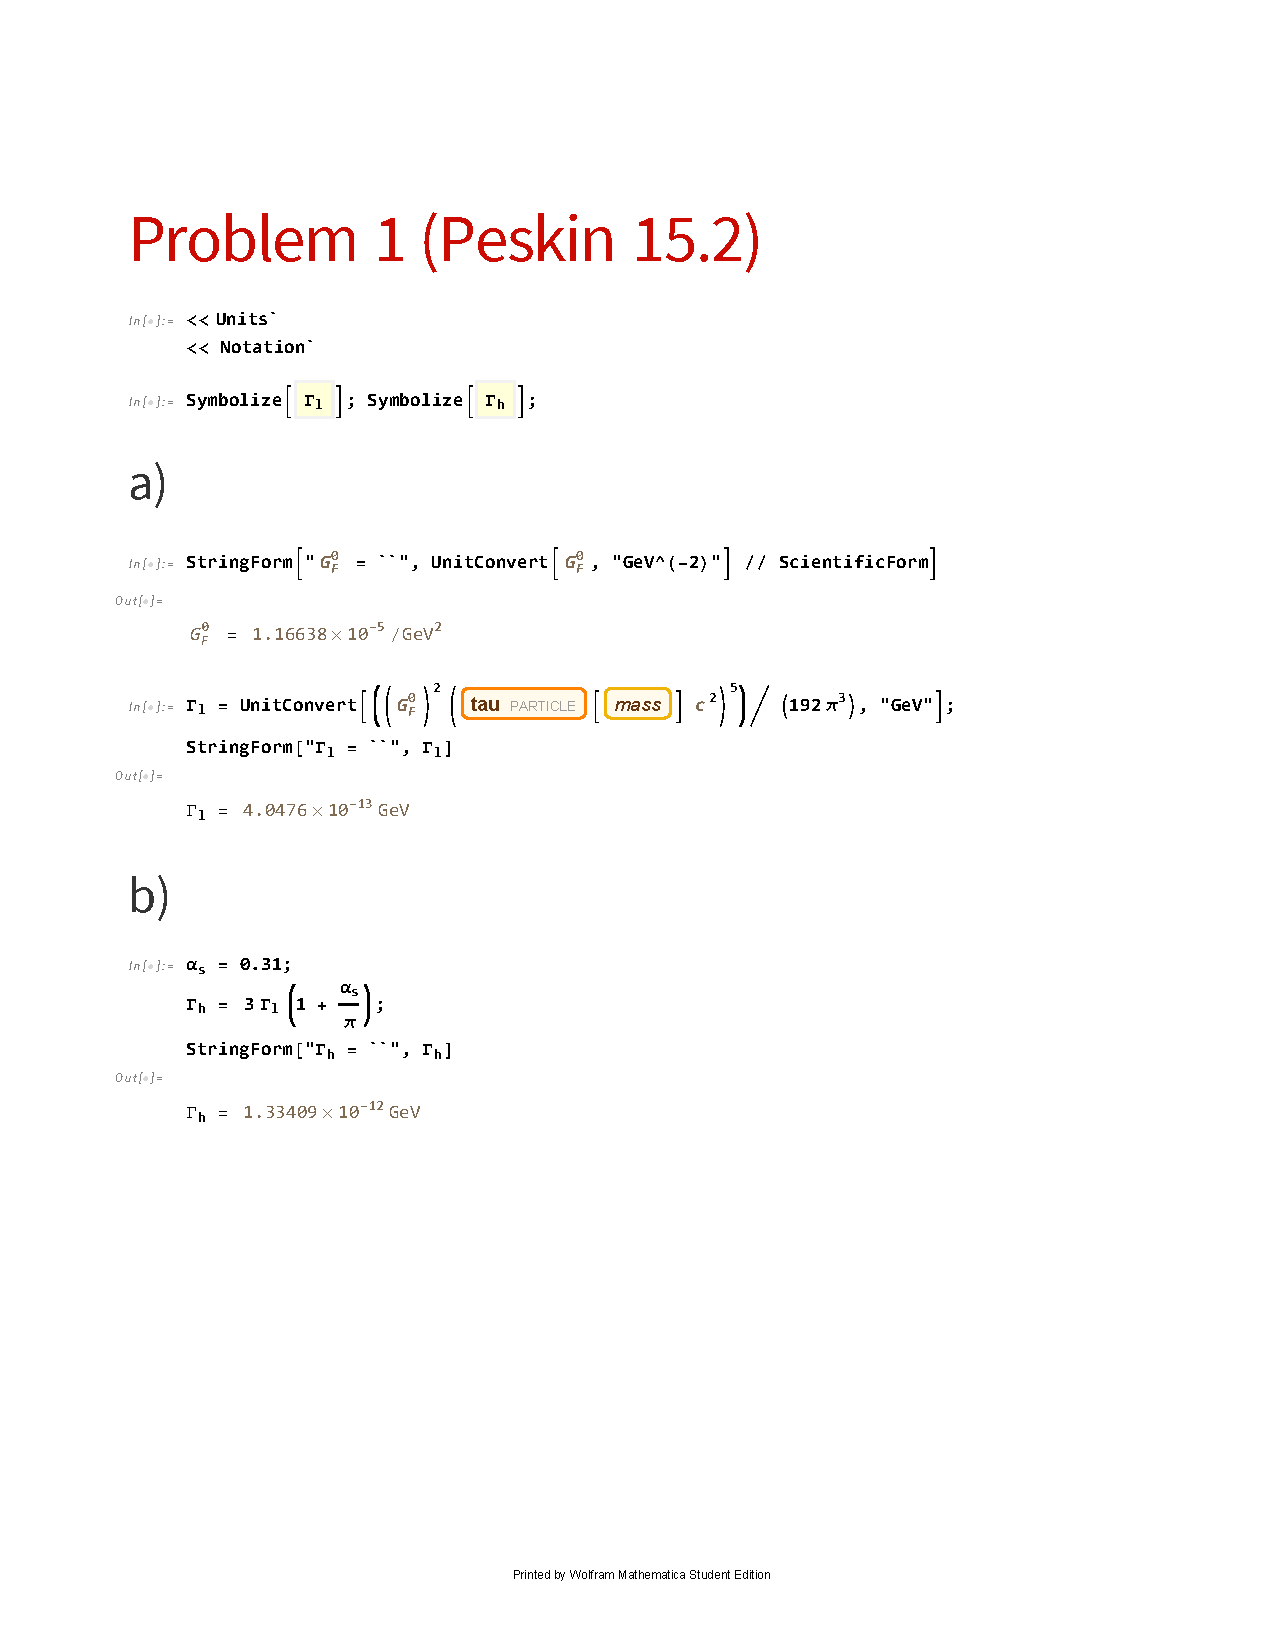
\includepdf[pages=-]{calcs/prob1.pdf}
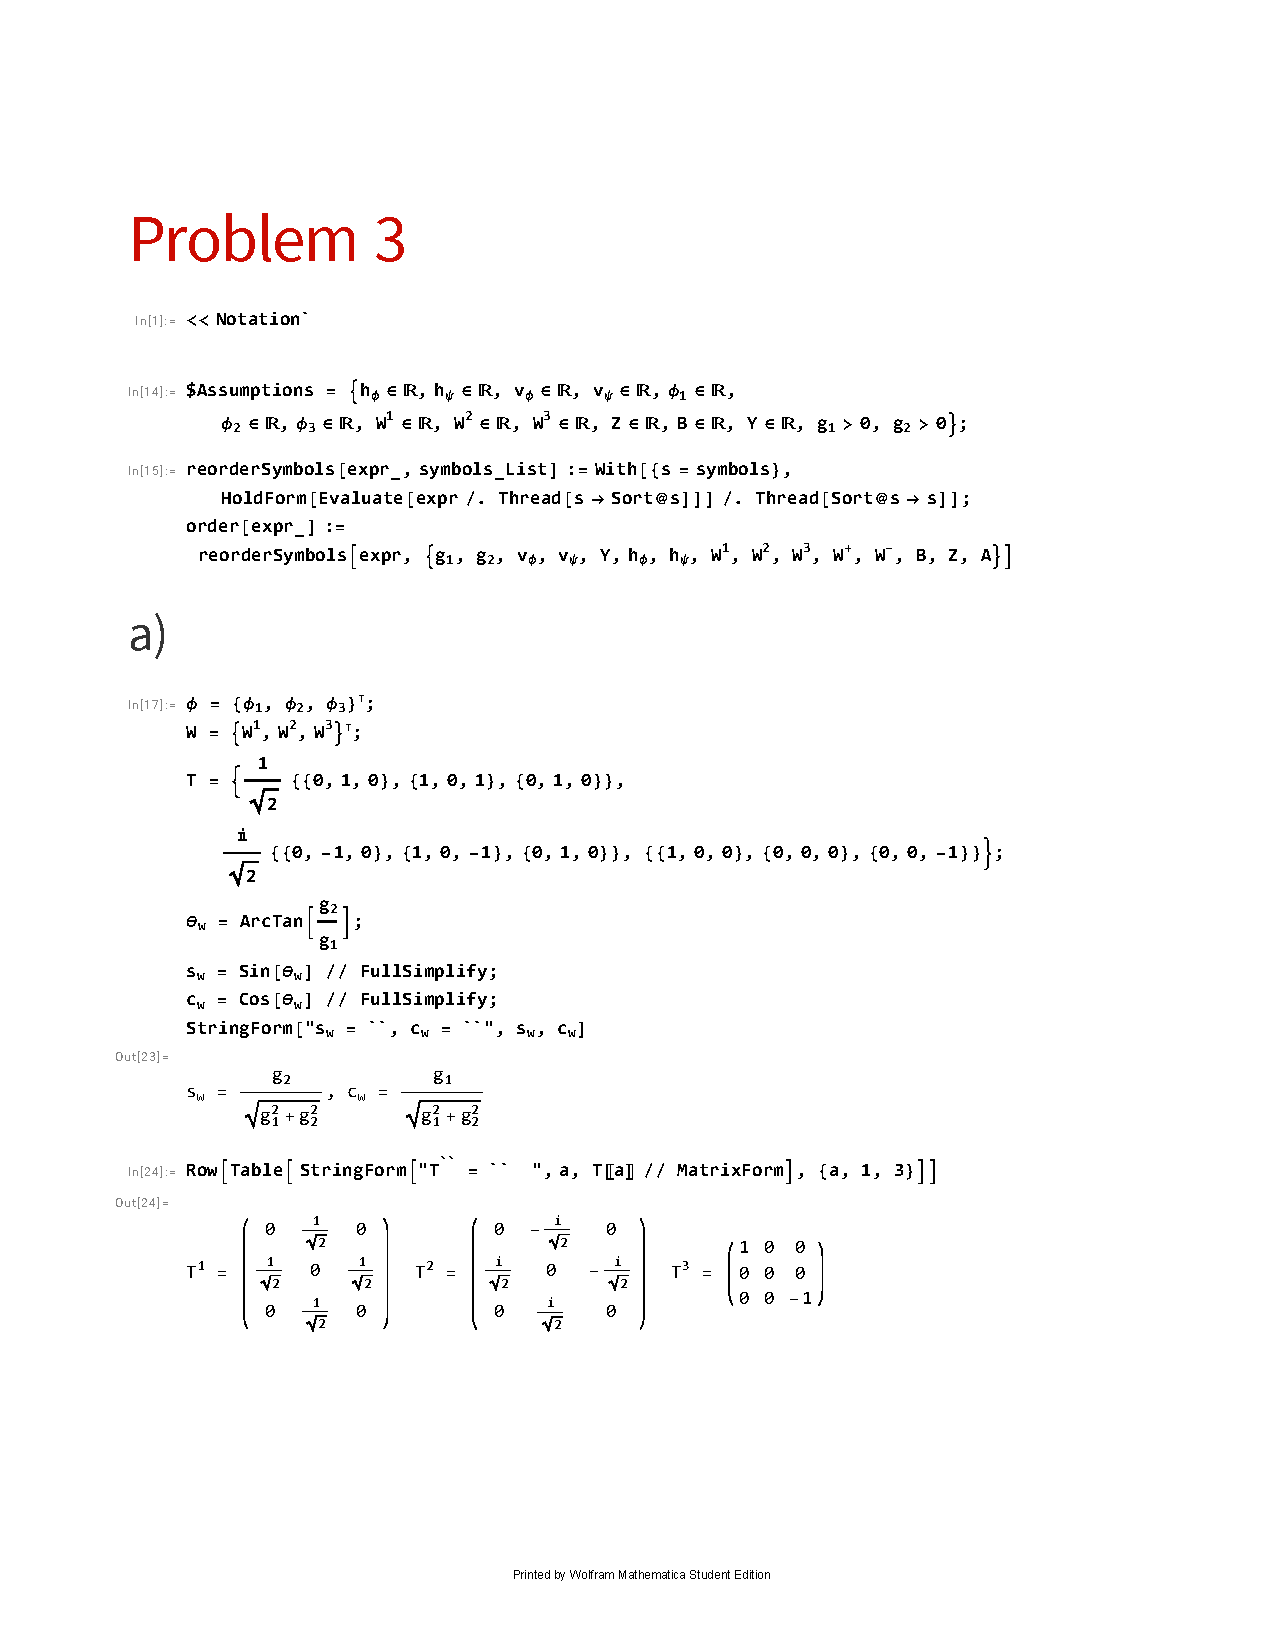
\includepdf[pages=-]{calcs/prob3.pdf}

\end{document}